\section{Reconmap's introduction}

\begin{frame}
    \frametitle{Section outline}

    \tableofcontents[currentsubsection, hideothersubsections, sectionstyle=show/hide]
\end{frame}

\subsection{Reconmap's mission}

\begin{frame}
    \frametitle{Reconmap mission}

    \note[item]{
    }
    
	\huge{\textbf{Reconmap} is making of \hl{every software engineer a penetration tester}}
\end{frame}

\begin{frame}
    \frametitle{Reconmap mission}

    \note[item]{
    }
    
    \centering
    
\includegraphics[scale=0.6]{oh-really.png}
\end{frame}

\begin{frame}
    \frametitle{Reconmap mission (continued)}

    \note[item]{
    }
    
    \begin{itemize}
    \item Make security testing more accessible
	\item Help (infosec)engineers collaborate better
    \item Accelerate project delivery
    \item Maximise returns
    \end{itemize}
\end{frame}

\begin{frame}
    \frametitle{What is Reconmap?}

    \note[item]{
    }
    
    \begin{outline}
	\1 Collaboration platform for InfoSec projects    
	\1 Automation and reporting tool for pentesters
	\1 Also...
    \2 Early-stage project
	\2 Open-source and SaaS
    \2 Developed in Dundee\footnotemark[1]
    \end{outline}
    
    \footnotetext[1]{with contributions from Argentina and the world}
\end{frame}

\begin{frame}
    \frametitle{Who is it for?}

    \note[item]{
    }
    
    \begin{outline}
	\1 InfoSec pros and teams looking to become more efficient
	\1 Other technical minded people\footnotemark[1] wanting to
	\2 Learn about security
    \2 Perform basic security on their projects
    \end{outline}
    
	\footnotetext[1]{devs, devops, it admins, sys admins, qa, etc...}
\end{frame}

\subsection{Features}

\begin{frame}
    \frametitle{Reconmap's functionality}

    \note[item]{
    }
    
    \begin{outline}
	\1 Project/Methodology templating
	\1 Task management
	\1 Shared space for
		\2 Files (docs, results, screenshots, etc)
		\2 Notes
	\1 Automation tool
    \end{outline}
\end{frame}


\begin{frame}
    \frametitle{Features}

    \note[item]{
    }
    
    \begin{outline}  		
    		\1 Database
    			\2 Commands
    			\2 Vulnerabilities
    			\2 Notes
    			
    		\1 Command automation
    		\1 Report generator
    \end{outline}
\end{frame}

\begin{frame}
    \frametitle{Commands}

    \note[item]{
    }
    \begin{columns}
		\begin{column}{0.5\textwidth}
			\begin{block}{Custom commands}
			\begin{itemize}
				\item Any arbitrary command
				\item Exec and dependencies installed by the user
				\item No upload integration
			\end{itemize}
			\end{block}
		\end{column}
		\begin{column}{0.5\textwidth}
			\begin{block}{Rmap commands}
			\begin{outline}
				\1 Container based
				\1 Dependencies included
	    			\1 Portable to Windows/Macos/Linux
	    			\1 Tighter integration with dashboard
		    \end{outline}
		    \end{block}
		\end{column}
	\end{columns}

\end{frame}

\begin{frame}
    \frametitle{Reconmap's code}

    \note[item]{
    }
    
	\begin{itemize}
		\item Open-source
		\item On Github $\rightarrow$ \url{https://github.com/reconmap}
		\item Easy to setup local environments
		\item Open for contributors
	\end{itemize}
\end{frame}

\subsection{Technical overview}

\begin{frame}
    \frametitle{Reconmap's architecture}

    \note[item]{
    }
    
	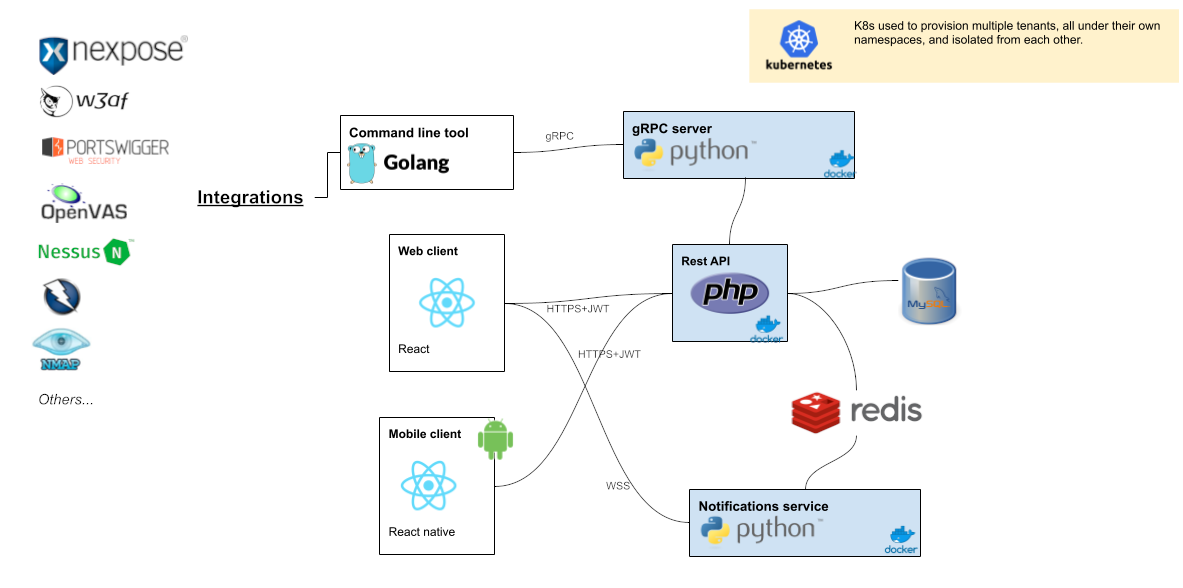
\includegraphics[]{reconmap-architecture.png}
\end{frame}

\begin{frame}
    \frametitle{API}

    \note[item]{
    }

	\begin{itemize}
		\item RESTful API
		\item OpenAPI specs
		\item Fully featured
		\item Used by CLI, Web and mobile clients
		\item \url{https://api.reconmap.org/docs/}
	\end{itemize}
\end{frame}

\subsection{Typical workflow}

\begin{frame}
    \frametitle{Typical workflow}

    \note[item]{
    }
    
    \begin{enumerate}
    \item Create client
    	\item Create project from template
    	\item Complete tasks
    	\item Some tasks require running commands
    	\item Reconmap (\textit{rmap}) runs the command, upload results, and analyses them
    	\item User annotates and triage vulnerabilities
    	\item Generate and share the report
    \end{enumerate}
\end{frame}

